% Peer joining

\label{sec:peer_joining}
\begin{figure*}
  %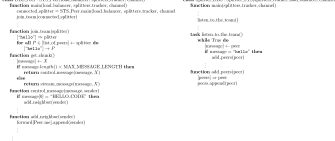
\includegraphics[width=\textwidth]{joining}
  \fig{230}{5cm}{joining}
  \caption{Tasks involved in a peer joining. $P^t_i$ is an incoming
    peer, and $P^t_k$ is a peer that is already in the team. $R$
    represents the tracker, and $S^t$ the splitter of the team $T^t$
    to which $P^t_i$ will be added.\label{fig:joining}}
\end{figure*}
An incoming peer $P^?_i$ (see the tasks described in
Fig.~\ref{fig:joining}), interested in a given channel, must first
join a team in order to access to the contents of such channel. For
that, $P^?_i$ requests a splitter to the \emph{tracker} $R$, with room
in its team ($R$ knows this information because each splitter sends to
$R$ the size of its teams when it changes). $R$ sends to $P^?_i$ a
\emph{reliable}\footnote{Reliable messages are transmitted over TCP
  and their transmission is denoted in the pseudocode by
  $\Rightarrow$. On the other hand, unreliable messages, which can be
  lost in transit, are transmitted over UDP and its transmission is
  denoted by $\rightarrow$. In any case, the reception of a packet is
  a permanent blocking action, at least a timeout is indicated.}
message $[S^t]$ (more exactly, the message transports the IP address
and port, i.e. an end-point, of the splitter $S^t$). Then, $P^?_i$
request to $S^t$ to be included in $T^t$. If $S^t$ accepts, then $S^t$
tranmits to $P^t_i$ the message $[T^t]$ (more preciselly, list of
peers in $T^t$, in a reliable message), and runs $T^t = T^t \cup
P^t_i$, in this order.
  %Then ${\cal P}_i$ polls
  %sequentially each splitter in $S$, requesting to be included in its
  %team until one of them (${\cal S}_j$, for example) accepts to ${\cal
  %  P}_i$. %Then, ${\cal S}_j$ performs ${\cal T}_j = {\cal T}_j \cup
  %{\cal P}_i$.  In parallel with the reception of $[{\cal T}_j]$,

While arriving, $P^t_i$ does not store $T^t$ as it is
received. Instead, for each $P^t_k\in [T^t]$, $P^t_i$ sends an
(unreliable) $[\mathtt{hello}]$ message to each $P^t_k$, and when
$P^t_k$ receives a $[\mathtt{hello}]$, it performs $T^t_k = T^t_k \cup
P^t_i$. Therefore, the list of peers $T^t_k$ that a peer $P^t_k$ has,
depends in first instance, on the number of $[\mathtt{hello}]$
messages that it has received. In other words, usually it holds that
$|T^t_k| \le |T^t|$.

% When a ${\cal P}_k$ receives a $[\mathtt{hello}]$ from ${\cal P}_i$,
% replies to ${\cal P}_i$ with the same message. -> Ya no hace falta
% porque los peers van a calcular las rutas óptimas al resto de peers
% del team con el flooding con poda.
% _________________________________________________________________
% Cuando un peer llega al team, envía los hello's y comienza a recibir
% chunks. Los peers por defecto reenvían todos los chunks recibidos al
% resto de peers, excepto al que se lo ha enviado. Por cada chunk
% recibido duplicado, los peers envía a quien se lo ha envíado un
% mensaje de prunning con un peer origen (el que figura en el chunk
% duplicado), indicando que no le envíe más chunks con ese
% origen. Cuando un peer eche de menos un chunk de un determinado peer
% origen (un determinado número de veces), enviará a uno o varios
% peers (en pricipio a todos los peers) del team un mensaje de
% revocación de prunning, para asegurarse de que aparece una mejor
% ruta alternativa para ese peer origen.
% __________________________________________________________________
%Then, ${\cal P}_i$ computes the RTT (Round-Trip Time) for each
%$[\mathtt{hello}]$ reply, and does $T^*({\cal P}_i) = T^*({\cal P}_i) \cup
%{\cal P}_k$, for those peers which reply
%%for the $K$ peers with lowest RTT
%($T^*({\cal
%  P}_i)$ is, by definition, the \emph{reacheable} team of ${\cal
%  P}_i$).
%%Later, all ${\cal P}_k\in N({\cal P}_i)$ performs $N({\cal
%%  P}_k) = N({\cal P}_k) \cup {\cal P}_i$, when a chunk of stream is
%%received from ${\cal P}_i$.
% __________________________________________________________________
% Ya no hace falta
% __________________________________________________________________

\begin{comment}
$[{\cal L}]=[\{{\cal X}\in {\cal T}^0/|N({\cal
    X})|<K\}]$ (being $K$ the maximum connectivity degree and $N({\cal
  X})$ the neighborhood of ${\cal X}$), and after that, ${\cal S}^0$
adds ${\cal P}$ to ${\cal T}^0$. In parallel with the reception of
$[{\cal L}]$, ${\cal P}$ sends a $[\mathtt{hello}]$ message to each
$\{{\cal X}\in {\cal T}^0\}$. When a ${\cal X}$ receives a
$[\mathtt{hello}]$, replies to ${\cal R}$ with the same message. Then,
${\cal X}$ computes a $\text{RTT}({\cal X})$ (Round-Trip Time) for
each $[\mathtt{hello}]$ reply, and sends to the $K$ peers with lowest
RTT
%$\underset{{\cal P}_i^0\in X}{\operatorname{{\it K}-first~args~min}} \,
%\text{RTT}({\cal P}_i^0)=\{K\text{-first}~{\cal P}_i^0~|~\forall
%     {\cal P}_j\in X:\text{RTT}({\cal P}_j)\leq \text{RTT}({\cal
%       P}_i)\}$,
a $[\mathtt{neighborhood\_request}]$ message, which ${\cal X}$ must
reply with a $[\mathtt{neighborhood\_accept}]$, if ${\cal X}$ accepts
${\cal P}$ as a neighbor. For each found neighbor ${\cal X}$, ${\cal
  P}$ sends to ${\cal S}^0$ a $[\mathtt{neighborhood\_accepted}~{\cal
    X}]$, and ${\cal S}^0$ updates $N({\cal P}) = N({\cal P}) \cup
\{{\cal X}\}$.
\end{comment}

% Ungraceful leaves occur when a peer leaves the group without
% notice which may cause disconnection of the peer’s descendants
% from the group.

% Ungraceful exit made by a peer may cause interruption of data
% reception at its descendants.
